\documentclass[border=4pt]{standalone}
\usepackage{tikz}
\usetikzlibrary{calc,shapes.geometric}

\begin{document}
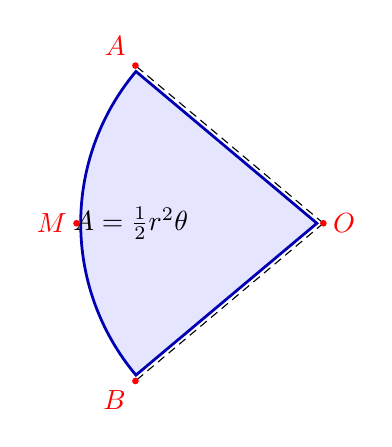
\begin{tikzpicture}
  \node[circular sector,circular sector angle=80,
    minimum width=36mm,minimum height=30mm,draw=blue!70!black,
    fill=blue!10,line width=1pt,outer sep=1.5pt] (S) at (0,0) {};
  \draw[densely dashed] (S.sector center) -- (S.arc start);
  \draw[densely dashed] (S.sector center) -- (S.arc end);
  \fill[red] (S.sector center) circle (1.2pt) node[right] {$O$};
  \fill[red] (S.arc start) circle (1.2pt) node[above left] {$A$};
  \fill[red] (S.arc center) circle (1.2pt) node[left] {$M$};
  \fill[red] (S.arc end) circle (1.2pt) node[below left] {$B$};
  \node at ($(S.center)+(-4mm,0)$) {$A=\frac{1}{2}r^2\theta$};
\end{tikzpicture}
\end{document}
